\documentclass[twoside]{book}

% Packages required by doxygen
\usepackage{fixltx2e}
\usepackage{calc}
\usepackage{doxygen}
\usepackage[export]{adjustbox} % also loads graphicx
\usepackage{graphicx}
\usepackage[utf8]{inputenc}
\usepackage{makeidx}
\usepackage{multicol}
\usepackage{multirow}
\PassOptionsToPackage{warn}{textcomp}
\usepackage{textcomp}
\usepackage[nointegrals]{wasysym}
\usepackage[table]{xcolor}

% NLS support packages
\usepackage[ngerman]{babel}

% Font selection
\usepackage[T1]{fontenc}
\usepackage[scaled=.90]{helvet}
\usepackage{courier}
\usepackage{amssymb}
\usepackage{sectsty}
\renewcommand{\familydefault}{\sfdefault}
\allsectionsfont{%
  \fontseries{bc}\selectfont%
  \color{darkgray}%
}
\renewcommand{\DoxyLabelFont}{%
  \fontseries{bc}\selectfont%
  \color{darkgray}%
}
\newcommand{\+}{\discretionary{\mbox{\scriptsize$\hookleftarrow$}}{}{}}

% Page & text layout
\usepackage{geometry}
\geometry{%
  a4paper,%
  top=2.5cm,%
  bottom=2.5cm,%
  left=2.5cm,%
  right=2.5cm%
}
\tolerance=750
\hfuzz=15pt
\hbadness=750
\setlength{\emergencystretch}{15pt}
\setlength{\parindent}{0cm}
\setlength{\parskip}{3ex plus 2ex minus 2ex}
\makeatletter
\renewcommand{\paragraph}{%
  \@startsection{paragraph}{4}{0ex}{-1.0ex}{1.0ex}{%
    \normalfont\normalsize\bfseries\SS@parafont%
  }%
}
\renewcommand{\subparagraph}{%
  \@startsection{subparagraph}{5}{0ex}{-1.0ex}{1.0ex}{%
    \normalfont\normalsize\bfseries\SS@subparafont%
  }%
}
\makeatother

% Headers & footers
\usepackage{fancyhdr}
\pagestyle{fancyplain}
\fancyhead[LE]{\fancyplain{}{\bfseries\thepage}}
\fancyhead[CE]{\fancyplain{}{}}
\fancyhead[RE]{\fancyplain{}{\bfseries\leftmark}}
\fancyhead[LO]{\fancyplain{}{\bfseries\rightmark}}
\fancyhead[CO]{\fancyplain{}{}}
\fancyhead[RO]{\fancyplain{}{\bfseries\thepage}}
\fancyfoot[LE]{\fancyplain{}{}}
\fancyfoot[CE]{\fancyplain{}{}}
\fancyfoot[RE]{\fancyplain{}{\bfseries\scriptsize Erzeugt von Doxygen }}
\fancyfoot[LO]{\fancyplain{}{\bfseries\scriptsize Erzeugt von Doxygen }}
\fancyfoot[CO]{\fancyplain{}{}}
\fancyfoot[RO]{\fancyplain{}{}}
\renewcommand{\footrulewidth}{0.4pt}
\renewcommand{\chaptermark}[1]{%
  \markboth{#1}{}%
}
\renewcommand{\sectionmark}[1]{%
  \markright{\thesection\ #1}%
}

% Indices & bibliography
\usepackage{natbib}
\usepackage[titles]{tocloft}
\setcounter{tocdepth}{3}
\setcounter{secnumdepth}{5}
\makeindex

% Hyperlinks (required, but should be loaded last)
\usepackage{ifpdf}
\ifpdf
  \usepackage[pdftex,pagebackref=true]{hyperref}
\else
  \usepackage[ps2pdf,pagebackref=true]{hyperref}
\fi
\hypersetup{%
  colorlinks=true,%
  linkcolor=blue,%
  citecolor=blue,%
  unicode%
}

% Custom commands
\newcommand{\clearemptydoublepage}{%
  \newpage{\pagestyle{empty}\cleardoublepage}%
}

\usepackage{caption}
\captionsetup{labelsep=space,justification=centering,font={bf},singlelinecheck=off,skip=4pt,position=top}

%===== C O N T E N T S =====

\begin{document}

% Titlepage & ToC
\hypersetup{pageanchor=false,
             bookmarksnumbered=true,
             pdfencoding=unicode
            }
\pagenumbering{roman}
\begin{titlepage}
\vspace*{7cm}
\begin{center}%
{\Large Physik-\/\+Engine \\[1ex]\large 0.\+0.\+0 }\\
\vspace*{1cm}
{\large Erzeugt von Doxygen 1.8.11}\\
\end{center}
\end{titlepage}
\clearemptydoublepage
\tableofcontents
\clearemptydoublepage
\pagenumbering{arabic}
\hypersetup{pageanchor=true}

%--- Begin generated contents ---
\chapter{R\+E\+A\+D\+ME}
\label{md_inc_3D_README}
\hypertarget{md_inc_3D_README}{}
T\+O\+DO 
\chapter{Physik-\/\+Engine v0.0.1 \mbox{[}!\mbox{[}Build Status\mbox{]}(https\+://travis-\/ci.org/tsteinholz/\+Physik-\/\+Engine.svg?branch=master)\mbox{]}(https\+://travis-\/ci.org/tsteinholz/\+Physik-\/\+Engine)}
\label{md_README}
\hypertarget{md_README}{}
\input{md_README}
\chapter{R\+E\+A\+D\+ME}
\label{md_src_3D_README}
\hypertarget{md_src_3D_README}{}
T\+O\+DO 
\chapter{Modul-\/\+Verzeichnis}
\section{Module}
Hier folgt die Aufzählung aller Module\+:\begin{DoxyCompactList}
\item \contentsline{section}{HÄ\+U\+F\+IG}{\pageref{group__H_xC3_x84UFIG}}{}
\begin{DoxyCompactList}
\item \contentsline{section}{M\+A\+T\+HE}{\pageref{group__MATHE}}{}
\begin{DoxyCompactList}
\item \contentsline{section}{V\+E\+K\+T\+O\+R2D}{\pageref{group__VEKTOR2D}}{}
\end{DoxyCompactList}
\end{DoxyCompactList}
\end{DoxyCompactList}

\chapter{Modul-\/\+Dokumentation}
\hypertarget{group__VEKTOR2D}{}\section{V\+E\+K\+T\+O\+R2D}
\label{group__VEKTOR2D}\index{V\+E\+K\+T\+O\+R2D@{V\+E\+K\+T\+O\+R2D}}
Zusammengehörigkeiten von V\+E\+K\+T\+O\+R2D\+:\nopagebreak
\begin{figure}[H]
\begin{center}
\leavevmode
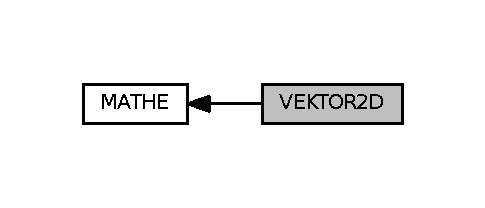
\includegraphics[width=233pt]{group__VEKTOR2D}
\end{center}
\end{figure}
\subsection*{Datenstrukturen}
\begin{DoxyCompactItemize}
\item 
struct \hyperlink{group__VEKTOR2D_structvektor2d__t}{vektor2d\+\_\+t}
\begin{DoxyCompactList}\small\item\em Eine Struktur 2D Vektor, der einen Koordinatenpunkt darstellt.  \hyperlink{group__VEKTOR2D_structvektor2d__t}{Mehr ...}\end{DoxyCompactList}\end{DoxyCompactItemize}
\begin{DoxyCompactItemize}
\item 
const \hyperlink{group__VEKTOR2D_structvektor2d__t}{vektor2d\+\_\+t} \hyperlink{group__VEKTOR2D_ga5261c4da7b847a8d2d91efd4cb9d0d17}{P\+H\+Y\+S\+I\+K\+\_\+\+E\+I\+N\+H\+E\+I\+T\+S\+\_\+\+V\+E\+K\+T\+O\+R2D}\hypertarget{group__VEKTOR2D_ga5261c4da7b847a8d2d91efd4cb9d0d17}{}\label{group__VEKTOR2D_ga5261c4da7b847a8d2d91efd4cb9d0d17}

\begin{DoxyCompactList}\small\item\em Die X und Y sind ein. \end{DoxyCompactList}\item 
const \hyperlink{group__VEKTOR2D_structvektor2d__t}{vektor2d\+\_\+t} \hyperlink{group__VEKTOR2D_ga1df5a950162dfc4005604d1618edee68}{P\+H\+Y\+S\+I\+K\+\_\+\+N\+U\+L\+L\+\_\+\+V\+E\+K\+T\+O\+R2D}\hypertarget{group__VEKTOR2D_ga1df5a950162dfc4005604d1618edee68}{}\label{group__VEKTOR2D_ga1df5a950162dfc4005604d1618edee68}

\begin{DoxyCompactList}\small\item\em Die X und Y sind null. \end{DoxyCompactList}\item 
const \hyperlink{group__VEKTOR2D_structvektor2d__t}{vektor2d\+\_\+t} \hyperlink{group__VEKTOR2D_gab758e3226f37fb0cc91cc382cd8ff4a1}{P\+H\+Y\+S\+I\+K\+\_\+\+Y\+\_\+\+V\+E\+K\+T\+O\+R2D}\hypertarget{group__VEKTOR2D_gab758e3226f37fb0cc91cc382cd8ff4a1}{}\label{group__VEKTOR2D_gab758e3226f37fb0cc91cc382cd8ff4a1}

\begin{DoxyCompactList}\small\item\em Die X sind null und die Y sind ein. \end{DoxyCompactList}\item 
const \hyperlink{group__VEKTOR2D_structvektor2d__t}{vektor2d\+\_\+t} \hyperlink{group__VEKTOR2D_gacc85ed6be7546dd40efbe1959419feed}{P\+H\+Y\+S\+I\+K\+\_\+\+X\+\_\+\+V\+E\+K\+T\+O\+R2D}\hypertarget{group__VEKTOR2D_gacc85ed6be7546dd40efbe1959419feed}{}\label{group__VEKTOR2D_gacc85ed6be7546dd40efbe1959419feed}

\begin{DoxyCompactList}\small\item\em Die X sind ein und die X sind null. \end{DoxyCompactList}\item 
\hyperlink{group__VEKTOR2D_structvektor2d__t}{vektor2d\+\_\+t} $\ast$ \hyperlink{group__VEKTOR2D_gaea1c504f3bee98b2bf6575c6fb80457d}{physik\+\_\+vektor2d\+\_\+hinzufugen} (\hyperlink{group__VEKTOR2D_structvektor2d__t}{vektor2d\+\_\+t} $\ast$a, \hyperlink{group__VEKTOR2D_structvektor2d__t}{vektor2d\+\_\+t} $\ast$b)
\item 
\hyperlink{group__VEKTOR2D_structvektor2d__t}{vektor2d\+\_\+t} $\ast$ \hyperlink{group__VEKTOR2D_gab8c1a14d4e4446abaaf017d8c520ab0d}{physik\+\_\+vektor2d\+\_\+subtrahieren} (\hyperlink{group__VEKTOR2D_structvektor2d__t}{vektor2d\+\_\+t} $\ast$a, \hyperlink{group__VEKTOR2D_structvektor2d__t}{vektor2d\+\_\+t} $\ast$b)
\item 
double \hyperlink{group__VEKTOR2D_ga1ce501d5038b8860e2b3fee21bb31a88}{physik\+\_\+vektor2d\+\_\+entfernung} (\hyperlink{group__VEKTOR2D_structvektor2d__t}{vektor2d\+\_\+t} $\ast$a, \hyperlink{group__VEKTOR2D_structvektor2d__t}{vektor2d\+\_\+t} $\ast$b)
\item 
void \hyperlink{group__VEKTOR2D_ga97e13e4933c07e7bd2cc10e95ea3dbc8}{physik\+\_\+skala\+\_\+vektor2d} (\hyperlink{group__VEKTOR2D_structvektor2d__t}{vektor2d\+\_\+t} $\ast$v, double skala)
\item 
\hyperlink{group__VEKTOR2D_structvektor2d__t}{vektor2d\+\_\+t} $\ast$ \hyperlink{group__VEKTOR2D_ga122ddb3ae52d3f0738672980869f8337}{physik\+\_\+vektor2d\+\_\+lerp} (\hyperlink{group__VEKTOR2D_structvektor2d__t}{vektor2d\+\_\+t} $\ast$v, \hyperlink{group__VEKTOR2D_structvektor2d__t}{vektor2d\+\_\+t} $\ast$ziel, double alpha)
\item 
void \hyperlink{group__VEKTOR2D_ga6f5b6b10e20fa779ea8c710fbe49fc6e}{physik\+\_\+vektor2d\+\_\+klemme} (\hyperlink{group__VEKTOR2D_structvektor2d__t}{vektor2d\+\_\+t} $\ast$v, double min, double max)
\end{DoxyCompactItemize}


\subsection{Ausführliche Beschreibung}
Definitionen für die 2\+D-\/\+Vektor. 

\subsection{Datenstruktur-\/\+Dokumentation}
\index{vektor2d\+\_\+t@{vektor2d\+\_\+t}}\label{structvektor2d__t}
\hypertarget{group__VEKTOR2D_structvektor2d__t}{}
\subsubsection{struct vektor2d\+\_\+t}
Eine Struktur 2D Vektor, der einen Koordinatenpunkt darstellt. 

Definiert in Zeile 54 der Datei vektor2\+D.\+h.

\begin{DoxyFields}{Datenstruktur-\/\+Elemente}
double\hypertarget{group__VEKTOR2D_abc6c2378cebc6d70131fe5ca1ff94050}{}\label{group__VEKTOR2D_abc6c2378cebc6d70131fe5ca1ff94050}
&
x&
Die X Koordinatenpunkt. \\
\hline

double\hypertarget{group__VEKTOR2D_a3c83744cd0477a439f4cd2385f702579}{}\label{group__VEKTOR2D_a3c83744cd0477a439f4cd2385f702579}
&
y&
Die Y Koordinatenpunkt. \\
\hline

\end{DoxyFields}


\subsection{Dokumentation der Funktionen}
\index{V\+E\+K\+T\+O\+R2D@{V\+E\+K\+T\+O\+R2D}!physik\+\_\+skala\+\_\+vektor2d@{physik\+\_\+skala\+\_\+vektor2d}}
\index{physik\+\_\+skala\+\_\+vektor2d@{physik\+\_\+skala\+\_\+vektor2d}!V\+E\+K\+T\+O\+R2D@{V\+E\+K\+T\+O\+R2D}}
\subsubsection[{\texorpdfstring{physik\+\_\+skala\+\_\+vektor2d(vektor2d\+\_\+t $\ast$v, double skala)}{physik_skala_vektor2d(vektor2d_t *v, double skala)}}]{\setlength{\rightskip}{0pt plus 5cm}void physik\+\_\+skala\+\_\+vektor2d (
\begin{DoxyParamCaption}
\item[{{\bf vektor2d\+\_\+t} $\ast$}]{v, }
\item[{double}]{skala}
\end{DoxyParamCaption}
)}\hypertarget{group__VEKTOR2D_ga97e13e4933c07e7bd2cc10e95ea3dbc8}{}\label{group__VEKTOR2D_ga97e13e4933c07e7bd2cc10e95ea3dbc8}
Waagen der Vektor der Komponenten. $(x * skala, y * skala)$


\begin{DoxyParams}{Parameter}
{\em } & \\
\hline
\end{DoxyParams}
\index{V\+E\+K\+T\+O\+R2D@{V\+E\+K\+T\+O\+R2D}!physik\+\_\+vektor2d\+\_\+entfernung@{physik\+\_\+vektor2d\+\_\+entfernung}}
\index{physik\+\_\+vektor2d\+\_\+entfernung@{physik\+\_\+vektor2d\+\_\+entfernung}!V\+E\+K\+T\+O\+R2D@{V\+E\+K\+T\+O\+R2D}}
\subsubsection[{\texorpdfstring{physik\+\_\+vektor2d\+\_\+entfernung(vektor2d\+\_\+t $\ast$a, vektor2d\+\_\+t $\ast$b)}{physik_vektor2d_entfernung(vektor2d_t *a, vektor2d_t *b)}}]{\setlength{\rightskip}{0pt plus 5cm}double physik\+\_\+vektor2d\+\_\+entfernung (
\begin{DoxyParamCaption}
\item[{{\bf vektor2d\+\_\+t} $\ast$}]{a, }
\item[{{\bf vektor2d\+\_\+t} $\ast$}]{b}
\end{DoxyParamCaption}
)}\hypertarget{group__VEKTOR2D_ga1ce501d5038b8860e2b3fee21bb31a88}{}\label{group__VEKTOR2D_ga1ce501d5038b8860e2b3fee21bb31a88}
Findet sich der Abstand zwischen zwei Vektoren. $\sqrt{(x_2-x_1)^2+(y_2-y_1)^2}$


\begin{DoxyParams}{Parameter}
{\em } & \\
\hline
\end{DoxyParams}
\index{V\+E\+K\+T\+O\+R2D@{V\+E\+K\+T\+O\+R2D}!physik\+\_\+vektor2d\+\_\+hinzufugen@{physik\+\_\+vektor2d\+\_\+hinzufugen}}
\index{physik\+\_\+vektor2d\+\_\+hinzufugen@{physik\+\_\+vektor2d\+\_\+hinzufugen}!V\+E\+K\+T\+O\+R2D@{V\+E\+K\+T\+O\+R2D}}
\subsubsection[{\texorpdfstring{physik\+\_\+vektor2d\+\_\+hinzufugen(vektor2d\+\_\+t $\ast$a, vektor2d\+\_\+t $\ast$b)}{physik_vektor2d_hinzufugen(vektor2d_t *a, vektor2d_t *b)}}]{\setlength{\rightskip}{0pt plus 5cm}{\bf vektor2d\+\_\+t}$\ast$ physik\+\_\+vektor2d\+\_\+hinzufugen (
\begin{DoxyParamCaption}
\item[{{\bf vektor2d\+\_\+t} $\ast$}]{a, }
\item[{{\bf vektor2d\+\_\+t} $\ast$}]{b}
\end{DoxyParamCaption}
)}\hypertarget{group__VEKTOR2D_gaea1c504f3bee98b2bf6575c6fb80457d}{}\label{group__VEKTOR2D_gaea1c504f3bee98b2bf6575c6fb80457d}
Fügen Sie zusammen zwei Vektoren. $(x_1 + x_2, y_1 + y_2)$


\begin{DoxyParams}{Parameter}
{\em } & \\
\hline
\end{DoxyParams}
\index{V\+E\+K\+T\+O\+R2D@{V\+E\+K\+T\+O\+R2D}!physik\+\_\+vektor2d\+\_\+klemme@{physik\+\_\+vektor2d\+\_\+klemme}}
\index{physik\+\_\+vektor2d\+\_\+klemme@{physik\+\_\+vektor2d\+\_\+klemme}!V\+E\+K\+T\+O\+R2D@{V\+E\+K\+T\+O\+R2D}}
\subsubsection[{\texorpdfstring{physik\+\_\+vektor2d\+\_\+klemme(vektor2d\+\_\+t $\ast$v, double min, double max)}{physik_vektor2d_klemme(vektor2d_t *v, double min, double max)}}]{\setlength{\rightskip}{0pt plus 5cm}void physik\+\_\+vektor2d\+\_\+klemme (
\begin{DoxyParamCaption}
\item[{{\bf vektor2d\+\_\+t} $\ast$}]{v, }
\item[{double}]{min, }
\item[{double}]{max}
\end{DoxyParamCaption}
)}\hypertarget{group__VEKTOR2D_ga6f5b6b10e20fa779ea8c710fbe49fc6e}{}\label{group__VEKTOR2D_ga6f5b6b10e20fa779ea8c710fbe49fc6e}
Beschränken Sie einen Vektor zu einem Bereich. $(min <= x <= max, min <= y <= max)$


\begin{DoxyParams}{Parameter}
{\em } & \\
\hline
\end{DoxyParams}
\index{V\+E\+K\+T\+O\+R2D@{V\+E\+K\+T\+O\+R2D}!physik\+\_\+vektor2d\+\_\+lerp@{physik\+\_\+vektor2d\+\_\+lerp}}
\index{physik\+\_\+vektor2d\+\_\+lerp@{physik\+\_\+vektor2d\+\_\+lerp}!V\+E\+K\+T\+O\+R2D@{V\+E\+K\+T\+O\+R2D}}
\subsubsection[{\texorpdfstring{physik\+\_\+vektor2d\+\_\+lerp(vektor2d\+\_\+t $\ast$v, vektor2d\+\_\+t $\ast$ziel, double alpha)}{physik_vektor2d_lerp(vektor2d_t *v, vektor2d_t *ziel, double alpha)}}]{\setlength{\rightskip}{0pt plus 5cm}{\bf vektor2d\+\_\+t}$\ast$ physik\+\_\+vektor2d\+\_\+lerp (
\begin{DoxyParamCaption}
\item[{{\bf vektor2d\+\_\+t} $\ast$}]{v, }
\item[{{\bf vektor2d\+\_\+t} $\ast$}]{ziel, }
\item[{double}]{alpha}
\end{DoxyParamCaption}
)}\hypertarget{group__VEKTOR2D_ga122ddb3ae52d3f0738672980869f8337}{}\label{group__VEKTOR2D_ga122ddb3ae52d3f0738672980869f8337}
Linear interpoliert zwischen zwei Vektoren. $y=y_0 + (y_1 - y_0)\tfrac{x-x_0}{x_1-x_0}$


\begin{DoxyParams}{Parameter}
{\em } & \\
\hline
\end{DoxyParams}
\index{V\+E\+K\+T\+O\+R2D@{V\+E\+K\+T\+O\+R2D}!physik\+\_\+vektor2d\+\_\+subtrahieren@{physik\+\_\+vektor2d\+\_\+subtrahieren}}
\index{physik\+\_\+vektor2d\+\_\+subtrahieren@{physik\+\_\+vektor2d\+\_\+subtrahieren}!V\+E\+K\+T\+O\+R2D@{V\+E\+K\+T\+O\+R2D}}
\subsubsection[{\texorpdfstring{physik\+\_\+vektor2d\+\_\+subtrahieren(vektor2d\+\_\+t $\ast$a, vektor2d\+\_\+t $\ast$b)}{physik_vektor2d_subtrahieren(vektor2d_t *a, vektor2d_t *b)}}]{\setlength{\rightskip}{0pt plus 5cm}{\bf vektor2d\+\_\+t}$\ast$ physik\+\_\+vektor2d\+\_\+subtrahieren (
\begin{DoxyParamCaption}
\item[{{\bf vektor2d\+\_\+t} $\ast$}]{a, }
\item[{{\bf vektor2d\+\_\+t} $\ast$}]{b}
\end{DoxyParamCaption}
)}\hypertarget{group__VEKTOR2D_gab8c1a14d4e4446abaaf017d8c520ab0d}{}\label{group__VEKTOR2D_gab8c1a14d4e4446abaaf017d8c520ab0d}
Subtrahieren zwei Vektoren. $(x_2 - x_1, y_2 - y_1)$


\begin{DoxyParams}{Parameter}
{\em } & \\
\hline
\end{DoxyParams}

\hypertarget{group__H_xC3_x84UFIG}{}\section{HÄ\+U\+F\+IG}
\label{group__H_xC3_x84UFIG}\index{HÄ\+U\+F\+IG@{HÄ\+U\+F\+IG}}
Zusammengehörigkeiten von HÄ\+U\+F\+IG\+:\nopagebreak
\begin{figure}[H]
\begin{center}
\leavevmode
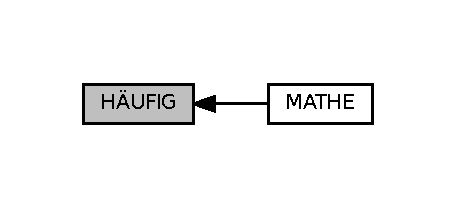
\includegraphics[width=219pt]{group__H_xC3_x84UFIG}
\end{center}
\end{figure}
\subsection*{Module}
\begin{DoxyCompactItemize}
\item 
\hyperlink{group__MATHE}{M\+A\+T\+HE}
\end{DoxyCompactItemize}


\subsection{Ausführliche Beschreibung}
Common Code für 2\+D-\/ und 3\+D-\/ pysics verwendet. 
\hypertarget{group__MATHE}{}\section{M\+A\+T\+HE}
\label{group__MATHE}\index{M\+A\+T\+HE@{M\+A\+T\+HE}}
Zusammengehörigkeiten von M\+A\+T\+HE\+:\nopagebreak
\begin{figure}[H]
\begin{center}
\leavevmode
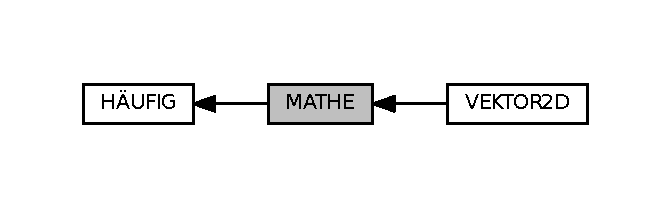
\includegraphics[width=322pt]{group__MATHE}
\end{center}
\end{figure}
\subsection*{Module}
\begin{DoxyCompactItemize}
\item 
\hyperlink{group__VEKTOR2D}{V\+E\+K\+T\+O\+R2D}
\end{DoxyCompactItemize}


\subsection{Ausführliche Beschreibung}
Mathematische Funktionen und definitons. 
%--- End generated contents ---

% Index
\backmatter
\newpage
\phantomsection
\clearemptydoublepage
\addcontentsline{toc}{chapter}{Index}
\printindex

\end{document}
